\documentclass[tikz,border=8pt]{standalone}
\usepackage{amsmath}
\usetikzlibrary{arrows.meta}

\definecolor{youngblue}{RGB}{31,104,157}
\definecolor{oldorange}{RGB}{181,92,41}
\definecolor{pricegray}{RGB}{82,82,82}
\definecolor{plangreen}{RGB}{67,130,89}

\begin{document}
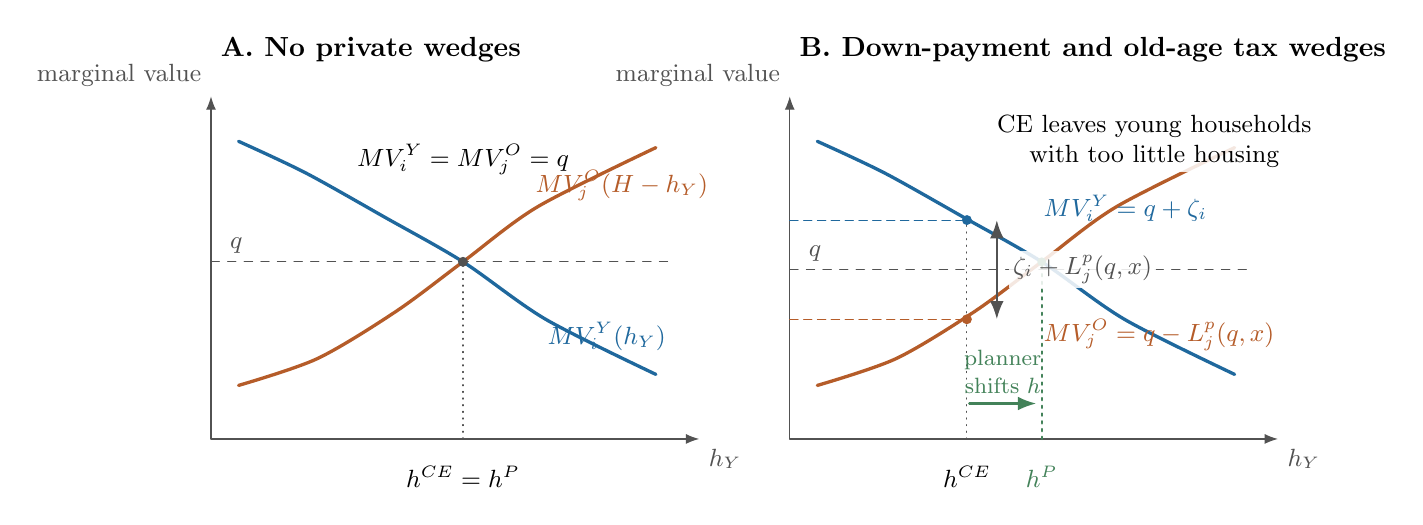
\begin{tikzpicture}[font=\small, >=Latex, line cap=round, line join=round]

% ---------- Panel A ----------
\begin{scope}[shift={(0,0)}]
  \node[anchor=west,font=\bfseries] at (0,4.95) {A. No private wedges};
  \draw[->,pricegray] (0,0) -- (6.2,0) node[below right] {$h_Y$};
  \draw[->,pricegray] (0,0) -- (0,4.35) node[above left] {marginal value};

  \draw[youngblue,very thick,smooth]
    plot coordinates {(0.35,3.78) (1.20,3.38) (2.20,2.82) (3.20,2.25) (4.25,1.52) (5.65,0.82)};
  \draw[oldorange,very thick,smooth]
    plot coordinates {(0.35,0.68) (1.35,1.02) (2.35,1.62) (3.20,2.25) (4.15,2.95) (5.65,3.70)};

  \draw[pricegray,dashed] (0,2.25) -- (5.85,2.25);
  \draw[pricegray,dotted] (3.20,0) -- (3.20,2.25);
  \fill[pricegray] (3.20,2.25) circle (1.8pt);

  \node[youngblue,anchor=west] at (4.15,1.30) {$MV_i^Y(h_Y)$};
  \node[oldorange,anchor=west] at (4.00,3.22) {$MV_j^O(H-h_Y)$};
  \node[pricegray,anchor=west] at (0.12,2.46) {$q$};
  \node[align=center,anchor=north] at (3.20,-0.22) {$h^{CE}=h^P$};
  \node[align=center] at (3.20,3.55)
    {$MV_i^Y=MV_j^O=q$};
\end{scope}

% ---------- Panel B ----------
\begin{scope}[shift={(7.35,0)}]
  \node[anchor=west,font=\bfseries] at (0,4.95) {B. Down-payment and old-age tax wedges};
  \draw[->,pricegray] (0,0) -- (6.2,0) node[below right] {$h_Y$};
  \draw[->,pricegray] (0,0) -- (0,4.35) node[above left] {marginal value};

  \draw[youngblue,very thick,smooth]
    plot coordinates {(0.35,3.78) (1.20,3.38) (2.20,2.82) (3.20,2.25) (4.25,1.52) (5.65,0.82)};
  \draw[oldorange,very thick,smooth]
    plot coordinates {(0.35,0.68) (1.35,1.02) (2.35,1.62) (3.20,2.25) (4.15,2.95) (5.65,3.70)};

  \draw[pricegray,dashed] (0,2.15) -- (5.85,2.15);
  \draw[pricegray,dotted] (2.25,0) -- (2.25,2.78);
  \draw[plangreen,dotted,thick] (3.20,0) -- (3.20,2.25);

  \fill[youngblue] (2.25,2.78) circle (1.8pt);
  \fill[oldorange] (2.25,1.52) circle (1.8pt);
  \fill[plangreen] (3.20,2.25) circle (1.6pt);

  \draw[youngblue,densely dashed] (0,2.78) -- (2.25,2.78);
  \draw[oldorange,densely dashed] (0,1.52) -- (2.25,1.52);
  \draw[<->,thick,pricegray] (2.63,1.52) -- (2.63,2.78)
    node[midway,right=4pt,align=left,fill=white,fill opacity=0.86,text opacity=1,inner sep=1.5pt]
    {$\zeta_i+L_j^p(q,x)$};

  \draw[->,thick,plangreen] (2.28,0.45) -- (3.13,0.45)
    node[midway,above,align=center] {\footnotesize planner\\[-1pt]\footnotesize shifts $h$};

  \node[pricegray,anchor=west] at (0.12,2.35) {$q$};
  \node[youngblue,anchor=west,align=left] at (3.10,2.93)
    {$MV_i^Y=q+\zeta_i$};
  \node[oldorange,anchor=west,align=left] at (3.10,1.32)
    {$MV_j^O=q-L_j^p(q,x)$};
  \node[align=center,anchor=north] at (2.25,-0.22) {$h^{CE}$};
  \node[plangreen,align=center,anchor=north] at (3.20,-0.22) {$h^P$};
  \node[align=center,fill=white,fill opacity=0.86,text opacity=1,inner sep=1.5pt] at (4.63,3.78)
    {CE leaves young households\\with too little housing};
\end{scope}

\end{tikzpicture}
\end{document}
